

\tikzset{every picture/.style={line width=0.75pt}} %set default line width to 0.75pt        

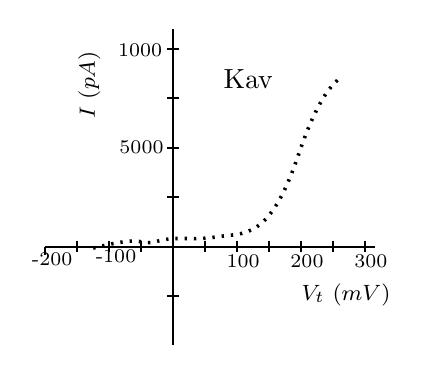
\begin{tikzpicture}[x=0.75pt,y=0.75pt,yscale=-0.7,xscale=0.7]
%uncomment if require: \path (0,300); %set diagram left start at 0, and has height of 300

%Straight Lines [id:da30256639311913547] 
\draw    (281.6,160.8) -- (496.6,160.8) -- (508.6,160.8) (303.6,156.8) -- (303.6,164.8)(325.6,156.8) -- (325.6,164.8)(347.6,156.8) -- (347.6,164.8)(369.6,156.8) -- (369.6,164.8)(391.6,156.8) -- (391.6,164.8)(413.6,156.8) -- (413.6,164.8)(435.6,156.8) -- (435.6,164.8)(457.6,156.8) -- (457.6,164.8)(479.6,156.8) -- (479.6,164.8)(501.6,156.8) -- (501.6,164.8) ;
%Straight Lines [id:da24911735771459287] 
\draw [line width=0.75]    (369.6,228.8) -- (369.6,10.8) (365.6,194.8) -- (373.6,194.8)(365.6,160.8) -- (373.6,160.8)(365.6,126.8) -- (373.6,126.8)(365.6,92.8) -- (373.6,92.8)(365.6,58.8) -- (373.6,58.8)(365.6,24.8) -- (373.6,24.8) ;
%Curve Lines [id:da6912957926978247] 
\draw  [dash pattern={on 0.84pt off 2.51pt}] [line width=1.3] (314.6,161.8) .. controls (354.6,151.8) and (343.72,161.07) .. (358.72,157.07) .. controls (373.72,153.07) and (380.72,157.07) .. (399.72,154.07) .. controls (418.72,151.07) and (435.72,157.07) .. (455.72,98.07) .. controls (475.72,39.07) and (487.72,49.07) .. (482.72,42.07) ;
%Straight Lines [id:da8823789696191159] 
\draw    (281.6,160.8) -- (281.6,166.8) ;

% Text Node
\draw (404.25,164.1) node [anchor=north west][inner sep=0.75pt]  [font=\scriptsize] [align=left] {100};
% Text Node
\draw (364.23,25.3) node [anchor=east] [inner sep=0.75pt]  [font=\scriptsize] [align=left] {1000};
% Text Node
\draw (314.25,161.1) node [anchor=north west][inner sep=0.75pt]  [font=\small] [align=left] {{\scriptsize -100}};
% Text Node
\draw (270.25,163.1) node [anchor=north west][inner sep=0.75pt]  [font=\small] [align=left] {{\scriptsize -200}};
% Text Node
\draw (312,75) node [anchor=west][inner sep=0.75pt]  [font=\footnotesize,rotate=-270] [align=left] {$\displaystyle I\ ( pA)$};
% Text Node
\draw (456,184) node [anchor=north west][inner sep=0.75pt]  [font=\footnotesize] [align=left] {$\displaystyle V_{t} \ ( mV)$};
% Text Node
\draw (402.2,37) node [anchor=north west][inner sep=0.75pt]   [align=left] {Kav};
% Text Node
\draw (365.23,92.3) node [anchor=east] [inner sep=0.75pt]  [font=\scriptsize] [align=left] {5000};
% Text Node
\draw (448.25,164.1) node [anchor=north west][inner sep=0.75pt]  [font=\scriptsize] [align=left] {200};
% Text Node
\draw (492.25,164.1) node [anchor=north west][inner sep=0.75pt]  [font=\scriptsize] [align=left] {300};


\end{tikzpicture}
